\chapter{Pointer subterfuge}

Il \textbf{pointer subterfuge} è un termine generale per gli exploit che modificano
il valore di un puntatore. In C e C++ esistono sia i puntatori a funzioni che i
puntatori a variabili.

\section{Puntatori a funzioni}

Nel caso dei puntatori a funzioni il valore di quest'ultimi può essere sovrascritto
in modo da trasferire il controllo a una shellcode fornita dall'attaccante.
Quando un programma esegue una  chiamata tramite il puntatore alla funzione, il codice
dell'attaccante è eseguito al posto del codice previsto.

\begin{figure}[H]
	\centering
	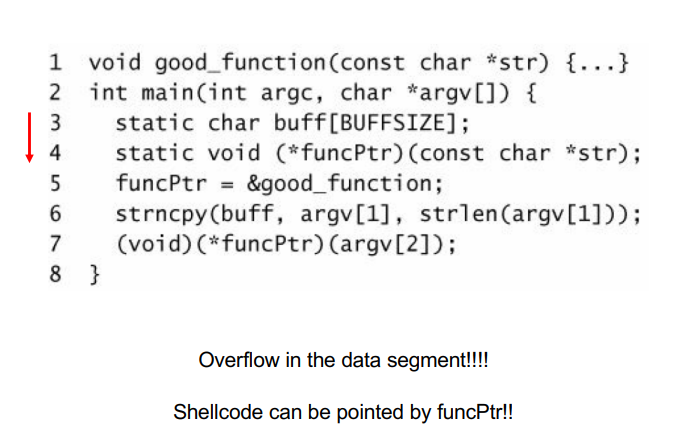
\includegraphics[width=10cm, keepaspectratio]{capitoli/secure_coding/img/cap_5/es_pointer_sub.png}
	\caption{Esempio pointer subterfuge su puntatori a funzioni.}\label{fig:es_poin_sub}
\end{figure}

Nel caso della Figura \ref{fig:es_poin_sub} il problema si trova nelle righe 3-4 poiché
non sappiamo la grandezza di \verb|BUFFSIZE| e questo può portare a un buffer overflow
sovrascrivendo il puntatore a funzione \verb|*funcPtr|. Abbiamo visto in precedenza
il buffer overflow applicato nello stack e nell'heap , in questo caso andiamo a
lavorare nella parte Data in cui vengono salvate le variabili sia globali che statiche.
Quindi le nostre variabili static \verb|buff[BUFFSIZE]| e \verb|*funcPtr| sono salvate,
presumibilmente una sotto l'altra, all'interno della parte Data della memoria.
In questo modo effettuando un buffer overflow si va a sovrascrivere il puntatore alla
funzione \verb|good_function| (riga 5), in seguito facendo uno \verb|strncpy| inserendo
più caratteri di quelli consentiti e richiamando la funzione tramite il suo
puntatore (riga 7) non si chiama effettivamente la \verb|good_function| ma
quello che abbiamo inserito noi.

\subsection{Puntatore a oggetti}

Lo stesso metodo può essere applicato ai puntatori a variabili.

\begin{figure}[H]
	\centering
	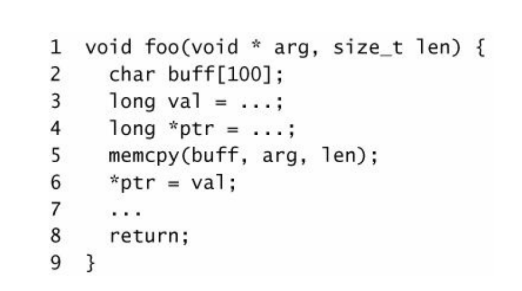
\includegraphics[width=10cm, keepaspectratio]{capitoli/secure_coding/img/cap_5/es_pointer_var.png}
	\caption{Esempio pointer subterfuge su puntatori a variabili.}\label{fig:es_poin_var}
\end{figure}

In questo caso abbiamo il \verb|buff[100]| di grandezza 100 caratteri seguito da
una variabile di tipo long e un puntatore sempre long. Nell'esempio di prima andavamo a
fare una \verb|strncpy| che portava al buffer overflow, qui invece facciamo
una \verb|memcpy(buff,arg,len)|\footnote{\textbf{void * memcpy ( void * destination,
		const void * source, size\_t num )}  Copia i valori dei byte di num, indica il numero di
	byte da copiare, dalla posizione a cui punta source direttamente nel blocco di memoria
	a cui punta destination.} che è sempre una copia non controllata da una zona sorgente
a una destinazione. Successivamente a riga 6 assegnando \verb|*ptr = val| scriviamo
un valore che vogliamo noi, poiché tramite il buffer overflow su buff[100] eccediamo
della grandezza massima e andiamo a sovrascrivere i valori delle successive variabili
a riga 3-4, in una zona di memoria che vogliamo noi quindi viene eseguita
una \textbf{scrittura di memoria arbitraria}.

\paragraph{Ultimo esempio}
Questo ultimo esempio differenzia da quelli precedenti per il modo in cui vengono
chiamate le funzioni, esse possono essere chiamate in modo diretto o indiretto.

\begin{figure}[H]
	\centering
	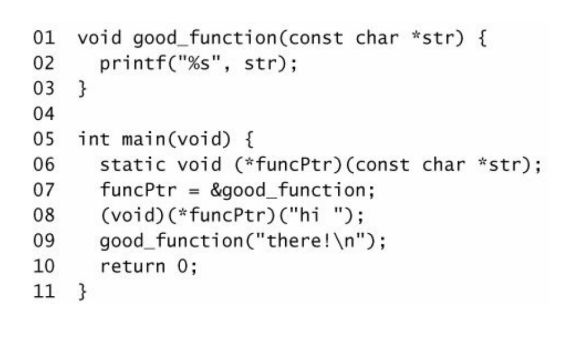
\includegraphics[width=10cm, keepaspectratio]{capitoli/secure_coding/img/cap_5/ult_es_point_sub.png}
	\caption{Esempio pointer subterfuge.}\label{fig:ult_es_poin}
\end{figure}

A riga 9 in Figura \ref{fig:ult_es_poin}possiamo vedere un esempio di chiamate diretta,
mentre a riga 8 abbiamo una indiretta poiché \verb|good_function| è chiamata tramite
il puntatore a quest'ultima. In Figura \ref{fig:dissas_ult_es_poin} vediamo a livello
assembly la differenza fra le due chiamate, la chiamate diretta è più semplice perché
viene effettuata, oltre la push per inserire nello stack la stringa da passare alla
funzione, direttamente una call a \textbf{good\_function}. Al contrario la chiamata
indiretta è un pò più complessa visto che non si fa una call
diretta a \textbf{good\_function} ma si chiama il puntatore a esse \verb|funcPtr|
che contiene l'indirizzo dove è salvata la funzione chiamata. L'istruzione di chiamata,
ad esempio, salva l'informazione di ritorno sullo stack e trasferisce il controllo
alla chiamata di funzione specificata dall'operando di destinazione (target). Il target
specifica l'indirizzo della prima istruzione nella funzione chiamata.

\begin{figure}[H]
	\centering
	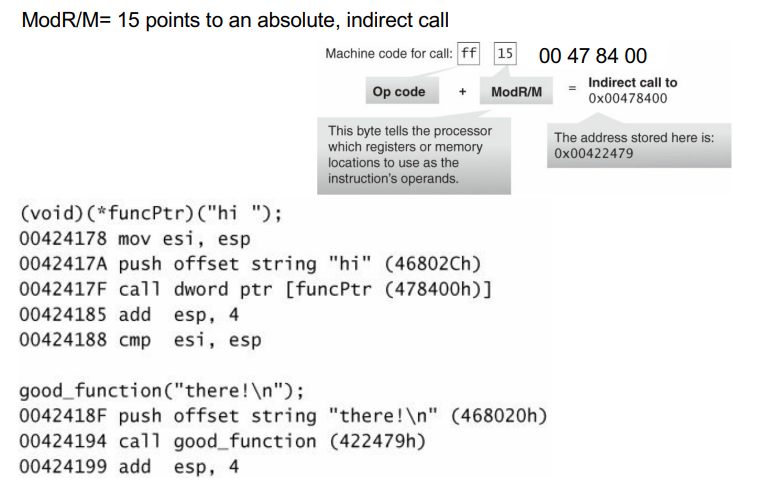
\includegraphics[width=12cm, keepaspectratio]{capitoli/secure_coding/img/cap_5/dissas_ult_es_point.png}
	\caption{Disassembly delle chiamate a \textbf{good\_function}.}\label{fig:dissas_ult_es_poin}
\end{figure}

Questo operando può essere un valore immediato, un registro generico, o una posizione
in memoria. Queste invocazioni di \textbf{good\_function()} forniscono esempi di
istruzioni di chiamata che possono e non possono essere attaccate. L'invocazione
statica utilizza un valore immediato come relativo spostamento, e questo spostamento
non può essere sovrascritto perché è nel segmento di codice. La chiamata tramite il
puntatore alla funzione utilizza un riferimento indiretto e l'indirizzo nella posizione
di riferimento può essere (in genere nel data o nel segmento dello stack) sovrascritto.
